\documentclass[conference,10pt]{IEEEtran}
\IEEEoverridecommandlockouts
\usepackage[utf8]{inputenc}
\usepackage[T1]{fontenc}
\usepackage[english]{babel}
\renewcommand{\figurename}{Figura}
\renewcommand{\tablename}{Tabla}
\usepackage{lmodern}
\usepackage{amsmath,amssymb}
\usepackage{graphicx}
\graphicspath{{./}{../capturas/}}
\usepackage{booktabs,tabularx,array,multirow}
\usepackage{tikz}
\usetikzlibrary{arrows.meta,positioning,shapes.geometric,fit}
\usepackage{pgfplots}
\pgfplotsset{compat=1.18}
\usepackage{xcolor}
\usepackage{url}
\usepackage{microtype}
\usepackage[hidelinks]{hyperref}
\usepackage{balance}
\renewcommand{\IEEEkeywordsname}{Palabras clave}
\definecolor{forest}{RGB}{11,42,26}
\definecolor{agold}{RGB}{172,139,73}
\newcolumntype{Y}{>{\raggedright\arraybackslash}X}
\newcommand{\ND}{\textit{Pend.}}
\newcommand{\ok}{\textbf{Aprob.}}
\begin{document}
\title{AGROPIDA: plataforma web para la trazabilidad del cuidado equino\\\large Diseño, análisis algorítmico y protocolo de evaluación mediante indicadores de negocio y tecnológicos}
\author{\IEEEauthorblockN{Alan Stanley Villalobos Bernal}
\IEEEauthorblockA{Proyecto académico AGROPIDA\\Bogotá D. C., Colombia}}
\maketitle
\renewcommand{\abstractname}{Resumen}
\begin{abstract}
La dispersión de registros relacionados con los ejemplares equinos dificulta consultar su identificación y organizar las actividades de cuidado. Este trabajo describe el diseño y la implementación de \emph{AGROPIDA}, un prototipo web dirigido al contexto del caballo de Paso Fino colombiano, con fichas de ejemplares, fotografías y eventos de salud, alimentación, entrenamiento y bienestar. Se presenta su arquitectura basada en HTML5, CSS3, JavaScript, \texttt{localStorage} e \texttt{IndexedDB}; se formalizan requisitos, historias de usuario, algoritmos y complejidad; y se propone un plan reproducible con cinco indicadores de negocio y cinco tecnológicos. La revisión del código y la ejecución local de cinco pruebas estructurales arrojaron cinco aprobaciones, pero no existe aún evidencia experimental de reducción de tiempos, mejora clínica ni cumplimiento de las metas de los diez indicadores. Se discuten los riesgos de almacenamiento local y autenticación demostrativa, y se delimitan futuras incorporaciones de trazabilidad centralizada y optimización. AGROPIDA se presenta como artefacto académico y no como sistema clínico validado.
\end{abstract}
\begin{IEEEkeywords}
gestión equina, trazabilidad, bienestar animal, aplicación web, indicadores KPI, evaluación de software.
\end{IEEEkeywords}
\renewcommand{\abstractname}{Abstract}
\begin{abstract}
Dispersed equine records can hinder animal identification, consultation, and the organization of care activities. This paper describes the design and implementation of \emph{AGROPIDA}, a web prototype for the Colombian Paso Fino context, featuring horse profiles, photographs, and records covering health, feeding, training, and welfare. The work reports a client-side architecture using HTML5, CSS3, JavaScript, \texttt{localStorage}, and \texttt{IndexedDB}; specifies requirements, user stories, algorithms, and computational complexity; and proposes a reproducible evaluation plan comprising five business and five technical KPIs. Source-code review and local execution of five structural tests resulted in five passes. However, no experimental evidence yet supports time savings, health outcomes, or achievement of the ten KPI targets. Limitations of local-only storage and demonstration authentication are discussed, along with prospective centralized traceability and optimization modules. AGROPIDA is an academic prototype rather than a clinically validated system.
\end{abstract}
\noindent\textbf{Index Terms---}equine management, traceability, animal welfare, web application, key performance indicators, software evaluation.

\section{Introducción}
La gestión de ejemplares equinos exige mantener disponibles datos de identificación, responsables, actividades de cuidado y antecedentes. Una dificultad operativa frecuente es la dispersión de dicha información en apuntes o archivos independientes; esta motivación es una \emph{hipótesis de problema} del proyecto que debe verificarse con usuarios, no una prevalencia nacional estimada. Como contexto sectorial, el Instituto Colombiano Agropecuario (ICA) informó una población de \textbf{1.482.286 equinos en Colombia en 2024} [1]. Este valor describe el inventario sectorial y \emph{no} cuantifica cuántos criaderos sufren problemas de registros.

La Organización Mundial de Sanidad Animal (OMSA/WOAH) considera el acceso al agua, la alimentación apropiada y la atención sanitaria aspectos relevantes del bienestar de los équidos en su ámbito normativo [2]. AGROPIDA busca apoyar el trabajo administrativo asociado a esos cuidados mediante una interfaz de consulta y registro. La contribución de este artículo es: a) documentar lo efectivamente implementado; b) distinguirlo de algoritmos propuestos; y c) diseñar un protocolo de validación trazable con metas medibles.

\section{Justificación}
La centralización de fichas y eventos, aunque sea en una primera interfaz local, ofrece un punto de partida para estandarizar nombres de campos, estados y procedimientos. En un escenario de criadero, consultar oportunamente una ficha o localizar un evento de cuidado podría reducir reprocesos y omisiones; su efecto real requiere una comparación empírica con el método habitual. La prioridad no es automatizar decisiones veterinarias, sino \textbf{organizar información} que el responsable puede revisar con profesionales competentes. La justificación integra el valor administrativo, la relevancia nacional de la actividad equina [1] y la necesidad de evaluar calidad de software de forma sistemática conforme al enfoque ISO/IEC 25010:2023 [3].

\section{Marco teórico}
\subsection{Trazabilidad y bienestar equino}
Se entiende por trazabilidad administrativa la posibilidad de relacionar un ejemplar identificado con registros fechados y categorizados. No equivale a una historia clínica certificada ni a sistemas nacionales oficiales. La guía de la OMSA para équidos de trabajo enfatiza agua, nutrición, salud y personal capacitado [2]; aquí se retoman como \emph{referentes conceptuales}, sin inferir que todas sus disposiciones aplican de idéntica forma al Paso Fino deportivo.

\subsection{Persistencia local y calidad del producto}
\texttt{localStorage} guarda cadenas asociadas a un origen web; los datos permanecen en ese navegador salvo eliminación o restricciones del entorno [4]. \texttt{IndexedDB} proporciona almacenamiento estructurado local apropiado para objetos y archivos como fotografías [5]. Estos mecanismos evitan un servidor en la primera versión, pero \textbf{no proporcionan sincronización entre usuarios}, control institucional de acceso ni copias centralizadas. La calidad de producto se evalúa con atributos pertinentes de ISO/IEC 25010 [3]; accesibilidad se aborda tomando WCAG 2.2 como referente [6].

\subsection{Métricas y medición}
La evaluación diferencia \emph{resultado observado}, \emph{meta propuesta} y \emph{dato pendiente}. Las métricas de experiencia web \emph{Largest Contentful Paint} (LCP), \emph{Interaction to Next Paint} (INP) y \emph{Cumulative Layout Shift} (CLS) usan umbrales recomendados de 2,5 s, 200 ms y 0,1, respectivamente, al percentil 75 [7]. Para usabilidad se propone \emph{System Usability Scale} (SUS), instrumento de diez ítems que proporciona puntuación de 0 a 100 [8]. Ninguna de estas mediciones se deduce de la inspección estática del código.

\section{Estado del arte y marco comparativo}
Existen soluciones comerciales orientadas a establos. \emph{Stable Secretary}, por ejemplo, publicita almacenamiento de registros identificativos, sanitarios, de herrador y de servicios, junto con herramientas de comunicación [9]. AGROPIDA no debe presentarse como el primer sistema de su tipo: su alcance diferencial en esta entrega es una interfaz demostrativa en español enfocada en el contexto colombiano, que prioriza el registro inicial de ejemplares y eventos de cuidado. La Tabla~\ref{tab:comparativo} contrasta funcionalidades \emph{declaradas} y alcance verificado del prototipo, no desempeño comparado.

\begin{table}[!t]
\caption{Comparación funcional cualitativa; información pública y código de AGROPIDA.}
\label{tab:comparativo}
\centering\footnotesize
\begin{tabularx}{\columnwidth}{@{}p{2.0cm}YY@{}}\toprule
\textbf{Característica}&\textbf{Stable Secretary [9]}&\textbf{AGROPIDA v1.0}\tabularnewline\midrule
Ficha del ejemplar&Disponible&Disponible\tabularnewline
Registros sanitarios&Disponible&Eventos de tipo ``Salud''\tabularnewline
Fotos y ficha visual&Disponible&Disponible, local\tabularnewline
Consulta compartida&Plataforma comercial&No implementada\tabularnewline
Veterinaria automatizada&No evaluada aquí&No implementada\tabularnewline
Población objetivo&Gestión de establos&Prototipo Paso Fino\tabularnewline\bottomrule
\end{tabularx}
\end{table}

\section{Diseño del sistema}
\subsection{Requisitos funcionales y no funcionales}
La Tabla~\ref{tab:req} sintetiza requisitos de producto: ``implementado'' significa identificable en el código fuente, no que el requisito haya aprobado una prueba funcional de extremo a extremo.

\begin{table*}[!t]
\caption{Requisitos, criterios de aceptación y estado de la versión examinada.}
\label{tab:req}
\centering\footnotesize
\begin{tabularx}{\textwidth}{@{}p{1cm}p{1cm}Y p{5.9cm} p{1.6cm}@{}}\toprule
\textbf{ID}&\textbf{Clase}&\textbf{Requisito}&\textbf{Criterio de aceptación propuesto}&\textbf{Estado}\tabularnewline\midrule
RF-01&Func.&Abrir acceso demostrativo y cambiar entre ingreso/registro.&Ingresar con datos ficticios sin errores de interfaz.&Implementado\tabularnewline
RF-02&Func.&Crear fichas con código y nombre obligatorios.&Rechazar duplicados y guardar ficha válida.&Implementado\tabularnewline
RF-03&Func.&Consultar y filtrar fichas existentes.&Buscar por código, nombre, responsable o color.&Implementado\tabularnewline
RF-04&Func.&Adjuntar y recuperar fotografía del ejemplar.&Visualizar imagen tras recarga en el mismo navegador.&Implementado\tabularnewline
RF-05&Func.&Registrar eventos de cuidado con fecha y categoría.&Almacenar evento válido asociado a un caballo.&Implementado\tabularnewline
RF-06&Func.&Visualizar y completar eventos pendientes.&El estado cambia y permanece tras recarga local.&Implementado\tabularnewline
RF-07&Func.&Presentar panel y conteos resumidos.&Los conteos concuerdan con el conjunto de prueba.&Implementado\tabularnewline
RF-08&Func.&Sincronizar entre usuarios y autenticar con servidor.&Datos y sesiones accesibles mediante perfiles autorizados.&No implementado\tabularnewline\midrule
RNF-01&No func.&Interfaz adaptable a escritorio y móvil.&Sin bloqueos visuales a anchos definidos en prueba.&Por validar\tabularnewline
RNF-02&No func.&Renderizado rápido.&LCP p75 $\leq 2{,}5$ s [7].&Por medir\tabularnewline
RNF-03&No func.&Interacción fluida y diseño estable.&INP p75 $\leq 200$ ms; CLS p75 $\leq 0{,}1$ [7].&Por medir\tabularnewline
RNF-04&No func.&Integridad de persistencia local.&Recuperación correcta en $\geq99\%$ de escenarios.&Por medir\tabularnewline
RNF-05&No func.&Accesibilidad evaluable.&Revisión de criterios aplicables de WCAG 2.2 [6].&Por validar\tabularnewline
RNF-06&No func.&Protección de cuentas y datos sensibles.&Autenticación real, permisos y respaldo.&Pendiente futuro\tabularnewline\bottomrule
\end{tabularx}
\end{table*}

\subsection{Historias de usuario}
\textbf{HU-01 (cuidador):} ``Como cuidador quiero registrar un ejemplar con código único para consultar su ficha''. \emph{Aceptación:} código y nombre validados, rechazo de duplicado y aparición de tarjeta. \textbf{HU-02 (cuidador):} ``Quiero asociar un control a un ejemplar para rastrear lo realizado''. \emph{Aceptación:} tipo, fecha, descripción y estado quedan en su historial. \textbf{HU-03 (administrador):} ``Quiero distinguir eventos pendientes de completados para organizar el seguimiento''. \emph{Aceptación:} cambio de estado persiste tras recarga local. \textbf{HU-04 (docente evaluador):} ``Quiero recorrer una demostración sin credenciales reales para examinar sus módulos''. \emph{Aceptación:} datos ficticios, acceso al panel y módulos navegables. El rol docente es un escenario de evaluación; \textbf{no existe un módulo docente con permisos reales}.

\subsection{Arquitectura y flujo de información}
La Fig.~\ref{fig:arquitectura} separa entrega web, lógica de interfaz y persistencia de origen local; el flujo registra un identificador de ejemplar y vincula eventos por \texttt{horseId}. La Fig.~\ref{fig:flujo} presenta la ruta funcional básica.

\begin{figure*}[!t]
\centering
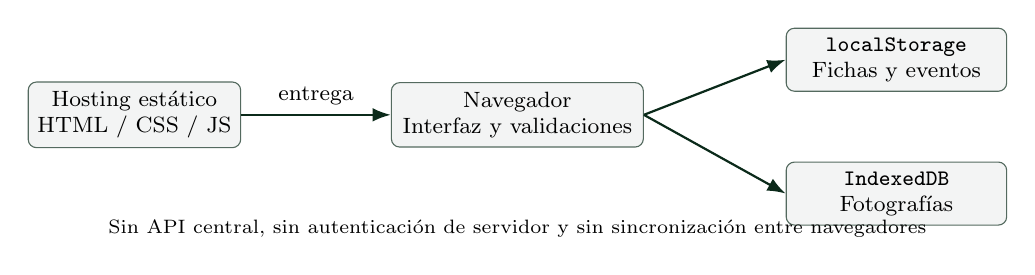
\begin{tikzpicture}[node distance=8mm and 10mm, every node/.style={font=\footnotesize}, arr/.style={-Latex,thick,draw=forest}, box/.style={draw=forest!70,rounded corners=3pt,minimum height=8mm,align=center,fill=forest!5}]
\node[box,minimum width=2.5cm] (host) {Hosting estático\\HTML / CSS / JS};
\node[box,minimum width=3.2cm,right=19mm of host] (browser) {Navegador\\Interfaz y validaciones};
\node[box,minimum width=2.8cm,right=18mm of browser,yshift=7mm] (local) {\texttt{localStorage}\\Fichas y eventos};
\node[box,minimum width=2.8cm,right=18mm of browser,yshift=-10mm] (idb) {\texttt{IndexedDB}\\Fotografías};
\draw[arr] (host) -- node[above]{entrega} (browser);
\draw[arr] (browser.east) -- (local.west);
\draw[arr] (browser.east) -- (idb.west);
\node[font=\scriptsize,below=8mm of browser,align=center] {Sin API central, sin autenticación de servidor y sin sincronización entre navegadores};
\end{tikzpicture}
\caption{Arquitectura real del prototipo AGROPIDA v1.0, derivada del código fuente.}
\label{fig:arquitectura}
\end{figure*}

\begin{figure}[!t]
\centering
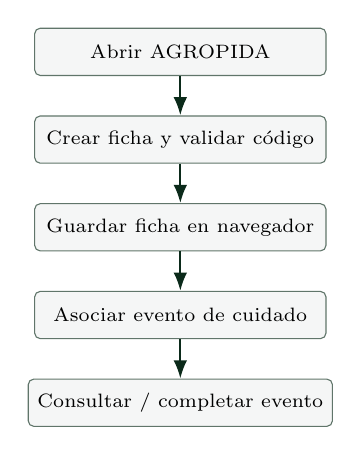
\begin{tikzpicture}[node distance=5mm, every node/.style={font=\scriptsize}, arr/.style={-Latex,thick,draw=forest},box/.style={draw=forest!65,rounded corners=2pt,fill=forest!4,align=center,minimum width=3.7cm,minimum height=6mm}]
\node[box] (a) {Abrir AGROPIDA};
\node[box,below=of a] (b) {Crear ficha y validar código};
\node[box,below=of b] (c) {Guardar ficha en navegador};
\node[box,below=of c] (d) {Asociar evento de cuidado};
\node[box,below=of d] (e) {Consultar / completar evento};
\foreach \x/\y in {a/b,b/c,c/d,d/e}{\draw[arr](\x)--(\y);}
\end{tikzpicture}
\caption{Flujo funcional observado en el código de AGROPIDA.}
\label{fig:flujo}
\end{figure}

\section{Algoritmos y análisis de complejidad}
\subsection{Procesos presentes en la implementación}
Sean $H$ el número de fichas y $R$ el número de eventos de cuidado; se asume longitud de texto acotada en el análisis dominante. El filtrado por nombre, código, responsable o pelaje recorre el arreglo de ejemplares, con costo $T_{\mathrm{buscar}}(H)=\Theta(H)$; la construcción de tarjetas es asimismo lineal en el número de resultados. La consulta de eventos emplea una copia y ordenamiento por fecha:
\begin{equation}
T_{\mathrm{ordenar}}(R)=O(R\log R),\qquad S(R)=O(R).
\label{eq:sort}
\end{equation}
El guardado serializa el conjunto de registros de cada navegador, con costo proporcional a su tamaño, idealmente $O(H+R)$ bajo registros de longitud acotada. La búsqueda de identificadores duplicados es $O(H)$; el detalle de un ejemplar combina una búsqueda lineal con filtrado y ordenación de su historial. En la rutina completa de renderizado, llamadas repetidas a búsquedas por identificador pueden incrementar el costo efectivo; no se afirma que exista una indexación optimizada. Las fotos se gestionan por operaciones asíncronas de \texttt{IndexedDB} [5].

\begin{table}[!t]
\caption{Complejidad asintótica de operaciones verificadas.}
\label{tab:comp}
\centering\footnotesize
\begin{tabularx}{\columnwidth}{@{}Yll@{}}\toprule
\textbf{Operación}&\textbf{Tiempo}&\textbf{Espacio aux.}\tabularnewline\midrule
Búsqueda de ficha&$O(H)$&$O(1)$\tabularnewline
Filtrar ejemplares&$O(H)$&$O(H)$\tabularnewline
Ordenar eventos&$O(R\log R)$&$O(R)$\tabularnewline
Guardar estado local&$O(H+R)$&$O(H+R)$\tabularnewline\bottomrule
\end{tabularx}
\end{table}

\subsection{Modelos algorítmicos propuestos, no implementados}
Por su mención en el planteamiento académico se discuten dos posibles extensiones. La \textbf{mochila 0/1} permitiría seleccionar actividades o materiales de capacitación bajo capacidad presupuestaria $C$: 
\begin{equation}
\max \sum_{i=1}^{n} v_ix_i\quad\mathrm{s.a.}\quad\sum_{i=1}^{n} c_ix_i\leq C,\ x_i\in\{0,1\}.
\label{eq:kp}
\end{equation}
Una programación dinámica sobre presupuesto entero ofrece $O(nC)$ tiempo y $O(C)$ memoria, complejidad seudopolinomial [10]. Los valores $v_i$ requerirían criterios explícitos; \emph{no} representan decisiones médicas automáticas.

El \emph{Bayesian Knowledge Tracing} (BKT) estima dominio de una habilidad de \textbf{personas en formación}, no salud equina [11]. Para una respuesta correcta y parámetros de deslizamiento $s$, adivinanza $g$ y probabilidad previa $p$: 
\begin{equation}
p^+=\frac{p(1-s)}{p(1-s)+(1-p)g},\qquad
p_{t+1}=p^++(1-p^+)\tau .
\label{eq:bkt}
\end{equation}
La actualización es $O(1)$ por interacción y $O(k)$ para $k$ respuestas. BKT solo tendría sentido en un \emph{futuro módulo formativo} de cuidadores o estudiantes. \textbf{Ni BKT ni mochila 0/1 aparecen en la versión HTML analizada}; sus modelos se incluyen como investigación futura, no como resultados.

\section{Implementación}
El repositorio organiza \texttt{index.html}, \texttt{src/styles.css}, \texttt{src/app.js}, imágenes de marca en \texttt{assets/}, documentación en \texttt{docs/} y pruebas en \texttt{tests/} [12]. La interfaz posee vistas de acceso demostrativo, tablero, ejemplares, registro, eventos, cuidados, orientación de texto y contacto. La versión examinada almacena datos estructurados en \texttt{localStorage}; las fotografías de usuario utilizan \texttt{IndexedDB}. Se aplican escapes al texto mostrado en HTML. El inicio de sesión acepta datos demostrativos y \textbf{no verifica contraseñas en un backend}; tampoco hay un modelo de IA conectado al apartado de consulta.

\begin{figure*}[!t]
\centering
\includegraphics[width=.87\textwidth]{inicio.png}
\caption{Captura real de la interfaz de inicio aportada por el equipo del proyecto: imagen del caballo azabache, identidad AGROPIDA y formulario de acceso de demostración.}
\label{fig:interfaz}
\end{figure*}

\section{Hipótesis e indicadores (KPIs)}
\subsection{Hipótesis operacionalizadas}
$H_1$: un flujo digital de registro permite reducir la mediana del tiempo por ficha al menos un 25\% respecto de un formulario manual equiparable. $H_2$: al finalizar un piloto controlado, al menos 90\% de los ejemplares de prueba tendrá ficha digital y al menos 95\% de las fichas evaluadas tendrá campos esenciales completos. $H_3$: la experiencia web satisface los umbrales técnicos propuestos. Las hipótesis son \emph{contrastables}, no resultados ya observados.

\subsection{Cinco KPIs de negocio}
La Tabla~\ref{tab:business} define denominadores auditables y metas \textbf{propuestas por el proyecto}, no estadísticas del sector. Para evitar resultados artificiales todos figuran como \emph{pendientes}; el indicador B3 requiere una bitácora externa usada solo como referencia experimental.
\begin{table*}[!t]
\caption{Cinco KPIs de negocio de AGROPIDA; metas definidas, mediciones de campo pendientes.}
\label{tab:business}
\centering\scriptsize
\begin{tabularx}{\textwidth}{@{}p{.48cm}p{2.55cm}Y p{1.85cm}p{3.0cm}p{.86cm}@{}}\toprule
\textbf{ID}&\textbf{Indicador / propósito}&\textbf{Definición y fórmula operacional}&\textbf{Meta y unidad}&\textbf{Fuente / periodicidad}&\textbf{Estado}\tabularnewline\midrule
B1&Cobertura de digitalización&$100\,H_{\rm digital}/H_{\rm inventario}$, inventario definido antes del piloto.&$\geq90\,\%$&Inventario de prueba versus fichas; al día 30.&\ND\tabularnewline
B2&Completitud de fichas&$100\,H_{\rm completas}/H_{\rm revisadas}$; código, nombre, responsable y campos pactados.&$\geq95\,\%$&Auditoría de fichas ficticias; semanal.&\ND\tabularnewline
B3&Trazabilidad del cuidado&$100\,R_{\rm documentados}/R_{\rm bit\acute{a}cora}$; mismas actividades e identificadores.&$\geq90\,\%$&Bitácora observacional de prueba; semanal.&\ND\tabularnewline
B4&Ahorro de tiempo administrativo&$100\,(\widetilde t_{\rm manual}-\widetilde t_{\rm web})/\widetilde t_{\rm manual}$; medianas apareadas.&$\geq25\,\%$&Cronometraje de la misma tarea; estudio piloto.&\ND\tabularnewline
B5&Usabilidad percibida&Escala SUS: diez ítems, puntuación de 0 a 100 puntos [8].&$\geq75$ puntos&Encuesta al terminar las tareas; cierre del piloto.&\ND\tabularnewline\bottomrule
\end{tabularx}
\end{table*}

\subsection{Cinco KPIs tecnológicos}
La Tabla~\ref{tab:technical} fija tres umbrales de Core Web Vitals recomendados por Google [7] y dos metas de verificación del proyecto. La distinción entre una prueba estructural y un KPI de campo evita confundir un test unitario con disponibilidad, rendimiento o éxito del usuario.
\begin{table*}[!t]
\caption{Cinco KPIs tecnológicos de AGROPIDA; criterios y medición propuesta.}
\label{tab:technical}
\centering\scriptsize
\begin{tabularx}{\textwidth}{@{}p{.48cm}p{2.45cm}Y p{1.83cm}p{3.1cm}p{.86cm}@{}}\toprule
\textbf{ID}&\textbf{Indicador / propósito}&\textbf{Definición y método de cálculo}&\textbf{Meta y unidad}&\textbf{Fuente / periodicidad}&\textbf{Estado}\tabularnewline\midrule
T1&Renderizado principal (LCP)&Percentil 75 de tiempo LCP en sesiones de prueba.&$\leq2{,}5$ s&Web Vitals / DevTools, móvil y escritorio.&\ND\tabularnewline
T2&Respuesta interactiva (INP)&Percentil 75 del retardo de interacciones observadas.&$\leq200$ ms&Instrumentación real de navegador; por sesión.&\ND\tabularnewline
T3&Estabilidad visual (CLS)&Percentil 75 de la puntuación acumulada de desplazamiento de diseño.&$\leq0{,}10$ (adim.)&Web Vitals, múltiples tamaños de pantalla.&\ND\tabularnewline
T4&Éxito de tareas críticas&$100\,N_{\rm tareas\;exitosas}/N_{\rm tareas\;intentadas}$ en flujo extremo a extremo.&$\geq95\,\%$&Guion de ejecución en navegadores; por versión.&\ND\tabularnewline
T5&Persistencia local correcta&$100\,N_{\rm restauraciones\;correctas}/N_{\rm escenarios\;guardados}$.&$\geq99\,\%$&Recarga de mismo origen/navegador; por versión.&\ND\tabularnewline\bottomrule
\end{tabularx}
\end{table*}

\section{Metodología de evaluación}
\subsection{Diseño del piloto}
Se propone una validación no clínica y observacional con al menos 12 participantes voluntarios (seis orientados a tareas de cuidado y seis evaluadores de interfaz), \emph{a reclutar}. Se utilizarán fichas y eventos totalmente ficticios, sin intervención en animales, bajo guion de tareas y consentimiento de quienes participen. Las tareas consisten en crear ficha, buscarla, adjuntar fotografía, registrar evento, completar estado y recargar. Para B4 se propone contrabalancear el orden manual/digital (secuencias AB/BA), medir tiempos en segundos, reportar mediana y rango intercuartílico; el efecto relativo se define en B4. B1--B3 requieren inventario y bitácora de referencia fijados \emph{antes} del estudio. Para B5 se administrará SUS después del uso [8].

\subsection{Procedimiento técnico y análisis}
Las pruebas de navegador se ejecutarán con datos de prueba en dos perfiles de equipo (escritorio y móvil) y al menos dos navegadores, con registro de versión, conectividad y dispositivo. T1--T3 se calcularán con muestras suficientes para p75, indicando tamaño real $n$; hasta entonces no puede afirmarse conformidad con Web Vitals. T4 se calcula sobre intentos de tareas completas; T5 comprueba persistencia en el mismo origen, nunca sincronización. Se define \emph{cumplimiento} por KPI como:
\begin{equation}
I_j=\begin{cases}1,&\text{si hay medida válida y supera la meta},\\0,&\text{si hay medida válida y no la supera},\\\text{ND},&\text{si todavía no hay medida.}\end{cases}
\end{equation}
Se reportarán denominadores, sesgos por muestra de conveniencia y fallos. Para hipótesis sobre medianas, el análisis podrá incluir intervalos de confianza por remuestreo, sujeto a suficiente tamaño muestral; con un piloto pequeño los resultados serán exploratorios.

\section{Resultados}
\subsection{Auditoría reproducible de ingeniería}
La revisión del artefacto local y la ejecución de \texttt{npm test} (Node.js) el 18 de noviembre de 2026 verificaron cinco comprobaciones estructurales del proyecto: enlaces a recursos, existencia de vistas, formularios, referencias a persistencia y presencia de recursos gráficos. El resultado fue \textbf{5 pruebas aprobadas de 5 ejecutadas (100\% de esta batería estructural)}. Esto \emph{no} indica 100\% de cobertura del código, ni cumplimiento de T4. La Fig.~\ref{fig:tests} muestra los cinco resultados binarios.
\begin{figure}[!t]
\centering
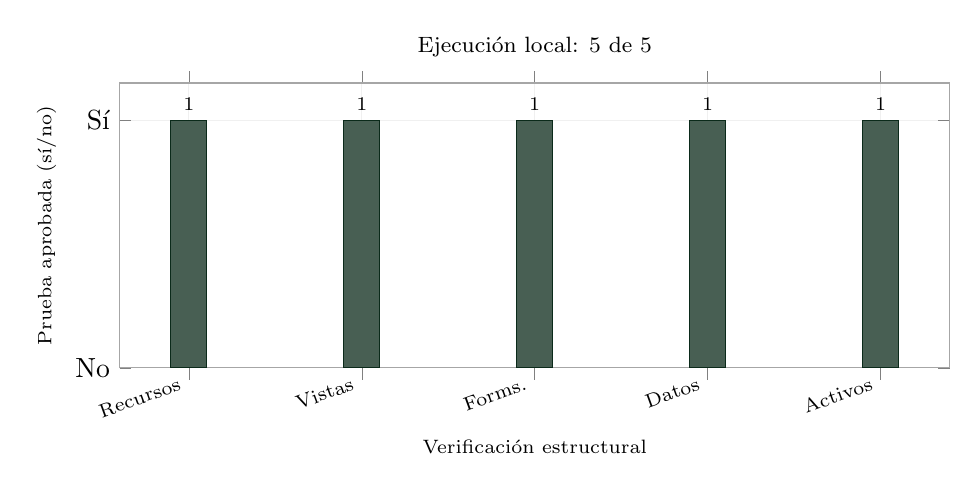
\begin{tikzpicture}
\begin{axis}[
width=\columnwidth,height=5.2cm,
ybar,bar width=13pt,
ymin=0,ymax=1.15,ytick={0,1},yticklabels={No, Sí},
xtick=data,xticklabels={Recursos,Vistas,Forms.,Datos,Activos},
x tick label style={font=\scriptsize,rotate=20,anchor=east},
ylabel={Prueba aprobada (sí/no)},xlabel={Verificación estructural},
label style={font=\scriptsize},title={Ejecución local: 5 de 5},title style={font=\footnotesize},
nodes near coords,point meta=y,nodes near coords style={font=\scriptsize},
grid=major,grid style={draw=gray!12},axis line style={draw=gray!70}]
\addplot[fill=forest!75,draw=forest] coordinates {(1,1) (2,1) (3,1) (4,1) (5,1)};
\end{axis}
\end{tikzpicture}
\caption{Resultados observados de pruebas de estructura ejecutadas localmente; una barra igual a 1 representa aprobación, no calidad clínica ni usabilidad.}
\label{fig:tests}
\end{figure}

\subsection{Indicadores de negocio y tecnología}
\textbf{No se dispone de datos de campo para B1--B5 o T1--T5.} Por tanto, se publican sus \emph{metas}, fórmulas y protocolos, pero \textbf{ningún porcentaje, puntaje SUS, tiempo LCP/INP ni reducción de tiempo se reporta como alcanzado}. La inspección confirma mecanismos de registro y persistencia en código; no verifica que los usuarios reales completen tareas ni que los datos sean compartidos. El sitio de demostración debe verificarse en acceso público antes de usar su URL como evidencia de disponibilidad.

\section{Análisis y discusión}
La principal fortaleza del prototipo es su trazabilidad administrativa básica: una ficha con identificador puede relacionarse con eventos de diferentes categorías, y la interfaz entrega información sin despliegue de backend. Su principal compromiso arquitectónico es la persistencia por navegador: resulta práctica para demostraciones individuales, pero imposibilita un historial institucional consistente, recuperación fiable entre dispositivos y control de permisos. Tampoco hay datos experimentales suficientes para sostener que la plataforma reduce errores de cuidado o mejora la salud de un animal. Comparada con una solución comercial como Stable Secretary [9], AGROPIDA cubre una fracción inicial del dominio y no acredita paridad en nube, colaboración y funcionalidades especializadas.

Los cinco KPIs de negocio evalúan adopción, calidad de registro, trazabilidad, eficiencia y percepción; los cinco tecnológicos analizan velocidad visual, respuesta, estabilidad, completitud de tareas y persistencia. Esa separación permite distinguir \emph{valor al criadero} de \emph{calidad de software}. La ausencia de mediciones no invalida la contribución de ingeniería, pero limita cualquier afirmación de efectividad. La Figura~\ref{fig:interfaz} es evidencia visual de diseño, no una prueba automática de usabilidad.

\section{Limitaciones y trabajos futuros}
\textbf{Limitaciones actuales:} almacenamiento en \texttt{localStorage} y \texttt{IndexedDB} sin servidor; autenticación y cuentas simuladas; ausencia de auditoría central y copias institucionales; consulta de IA no conectada; ausencia de validaciones de campo, seguridad, accesibilidad y rendimiento; evaluación comparativa funcional limitada a información pública. No existen aún módulos de estudiantes y docentes, BKT, optimización de mochila ni integración veterinaria certificada.

\textbf{Trabajo futuro:} i) migrar a API y base de datos transaccional con autenticación real, roles y auditoría; ii) incorporar backups, gestión de consentimiento y minimización de información; iii) implementar agenda con fecha programada, fecha de cumplimiento y alertas; iv) evaluar accesibilidad bajo WCAG 2.2 [6] y calidad según ISO/IEC 25010 [3]; v) completar piloto con medición formal de los diez KPIs; vi) explorar mochila 0/1 para asignación de recursos de capacitación, y BKT solamente si se incorpora un componente educativo con datos adecuados.

\section{Conclusiones}
AGROPIDA constituye un prototipo web coherente para fichas de ejemplares y documentación de eventos de cuidado de caballos en el contexto colombiano. La arquitectura cliente--navegador permite una demostración accesible y separa claramente vistas, lógica y recursos, pero no proporciona capacidades multiusuario, seguridad de producción o supervisión clínica. La revisión del código y cinco pruebas estructurales locales ofrecen evidencia \emph{limitada pero reproducible} de que el artefacto contiene los módulos y recursos esperados; no debe confundirse ese resultado con validación integral. Como aportación evaluativa, se formularon cinco KPIs de negocio y cinco técnicos con metas, unidades, denominadores, instrumentos y estado explícito, de forma que una siguiente fase pueda comprobar utilidad y desempeño sin inventar resultados. La estrategia responsable es evolucionar el prototipo hacia una arquitectura centralizada y contrastar sus beneficios mediante evaluación controlada con usuarios y datos ficticios, preservando la decisión profesional del cuidador y del veterinario.

\balance
\begin{thebibliography}{12}
\bibitem{ica} Instituto Colombiano Agropecuario (ICA), ``El ICA y Fedequinas comprometidos con el bienestar animal,'' 2024. [En línea]. Disponible: \url{https://www.ica.gov.co/noticias/ica-fedequinas-comprometidos-bienestar-animal-1}. [Consultado: 18-nov-2026].
\bibitem{woah} World Organisation for Animal Health, ``Terrestrial Animal Health Code, Ch. 7.12: Welfare of working equids,'' 2024. [En línea]. Disponible: \url{https://www.woah.org/fileadmin/Home/eng/Health_standards/tahc/current/en_chapitre_aw_working_equids.htm}. [Consultado: 18-nov-2026].
\bibitem{iso} ISO/IEC, \emph{ISO/IEC 25010:2023, Systems and software engineering---SQuaRE---Product quality model}, 2023. Disponible: \url{https://www.iso.org/standard/78176.html}.
\bibitem{mdnlocal} MDN Web Docs, ``Window: localStorage property.'' [En línea]. Disponible: \url{https://developer.mozilla.org/en-US/docs/Web/API/Window/localStorage}. [Consultado: 18-nov-2026].
\bibitem{mdnidb} MDN Web Docs, ``IndexedDB API.'' [En línea]. Disponible: \url{https://developer.mozilla.org/en-US/docs/Web/API/IndexedDB_API}. [Consultado: 18-nov-2026].
\bibitem{wcag} World Wide Web Consortium (W3C), \emph{Web Content Accessibility Guidelines (WCAG) 2.2}, 2023. Disponible: \url{https://www.w3.org/TR/WCAG22/}.
\bibitem{vitals} Google, ``Web Vitals,'' web.dev. [En línea]. Disponible: \url{https://web.dev/articles/vitals}. [Consultado: 18-nov-2026].
\bibitem{sus} J. Brooke, ``SUS: A quick and dirty usability scale,'' en \emph{Usability Evaluation in Industry}, P. W. Jordan \emph{et al.}, Eds. London, UK: Taylor \& Francis, 1996, pp. 189--194.
\bibitem{stable} Stable Secretary, ``Features: Equine and barn management software.'' [En línea]. Disponible: \url{https://stablesecretary.com/features/}. [Consultado: 18-nov-2026].
\bibitem{kp} University of Maryland, ``Lecture 31: Dynamic Programming: 0--1 Knapsack Problem,'' \emph{CMSC 451 lecture notes}, 2025. Disponible: \url{https://www.cs.umd.edu/class/spring2025/cmsc451-0101/Lects/cmsc451-spring25-lects.pdf}.
\bibitem{bkt} A. T. Corbett y J. R. Anderson, ``Knowledge tracing: Modeling the acquisition of procedural knowledge,'' \emph{User Modeling and User-Adapted Interaction}, vol. 4, pp. 253--278, 1994, doi: 10.1007/BF01099821.
\bibitem{repo} A. S. Villalobos Bernal, ``PR-AGROPIDA, código y documentación del prototipo,'' repositorio GitHub, versión 1.0, 2026. Disponible: \url{https://github.com/stanleey07/PR-AGROPIDA}. [Acceso sujeto a permisos del repositorio].
\end{thebibliography}
\end{document}